\section{パラメータの更新}
{第6章ではニューラルネットワークの学習において重要な役割を果たすパラメータについて学んだ。最適な重みパラメータを探索する最適化手法に始まり、重みパラメータの初期値、ハイパーパラメータの設定方法などである。そこで記されている手法を用いることでニューラルネットワーク(ディープラーニング)の学習を効率的に進めることができ、認識精度を高めることができる。
  \bunseki{※薩田凱斗}
}



\subsection{確率的勾配下降法}
{ニューラルネットワークにおける学習の目的は、損失関数の値をできるだけ小さくするパラーメータを見つけることであり、それを最適化という。最適化は非常に複雑で難解であるためパラメータの勾配を手がかりに探していく。これは確率的勾配下降法と言い非常に単純な最適化の手法である。確率的勾配下降法の数式は以下のように表される。
{
\begin{equation}
\label{eq1}
\bf W \leftarrow W - \eta  \frac{\partial L}{\partial W}
\end{equation}
}
ここで、更新する重みパラメータを{\bf W} 、{\bf W}に関する損失関数の勾配を$\displaystyle \frac{\partial L}{\partial W}$とする。$\displaystyle {\eta}$は学習係数を表し、あらかじめ決めておいた値を使用する。また、式中の$\displaystyle {\leftarrow}$は、右辺の値で左辺の値を更新するということを表している。式(\ref{eq1})で表されるように、確率的勾配下降法は勾配方向へある一定の距離だけ進むという単純な方法であることがわかった。しかし、この確率的勾配下降法には欠点がある。単純で実装も簡単という利点があるが、問題によっては非効率な場合が存在する。その欠点を指摘するために次の関数の最小値を求める問題を考える。
\begin{equation}
\label{eq2}
f(x,y) = \frac{1}{20}x^{2} + y^{2}
\end{equation}
式(\ref{eq2})で表される関数は図\ref{gr1}に示してあるような形状のグラフである。ここで、このグラフで表される関数の勾配を見ていく。
\begin{figure}[H]
\label{gr1}
\centering
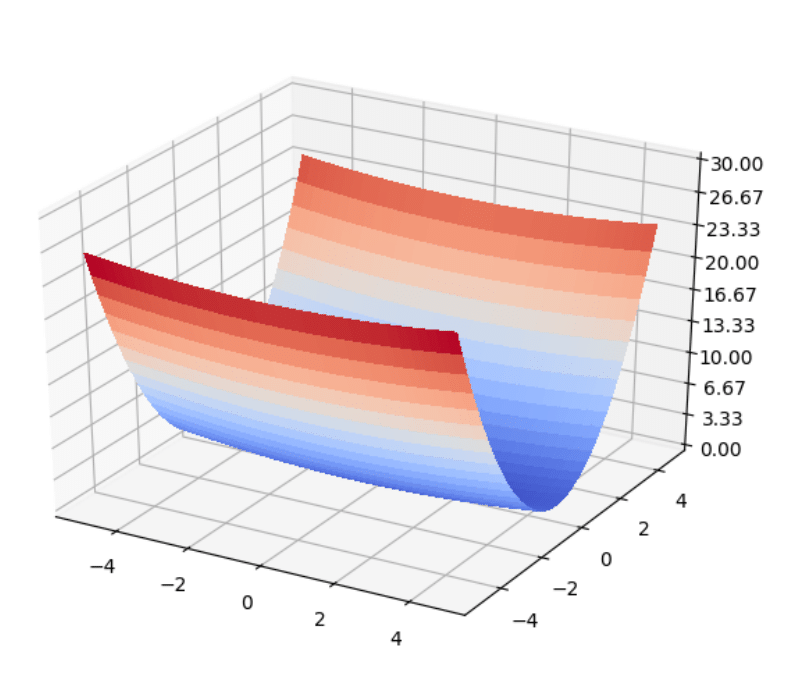
\includegraphics[width=6cm]{./figure/Graph.png}
\caption{$\displaystyle f(x,y) = \frac{1}{20}x^2 + y^2$のグラフ \label{gr1}}
\end{figure} 図1の形状の関数に対して確率的勾配下降法を適応してみる。探索の開始場所である初期値を$\displaystyle (x,y) = (-7.0, 2.0)$から始める。確率的勾配下降法は、図\ref{gr2}に表されるようなジグザグな動きをし、最小値に向かう動きとしてはかなり非効率な経路である。
\begin{figure}[H]
\centering
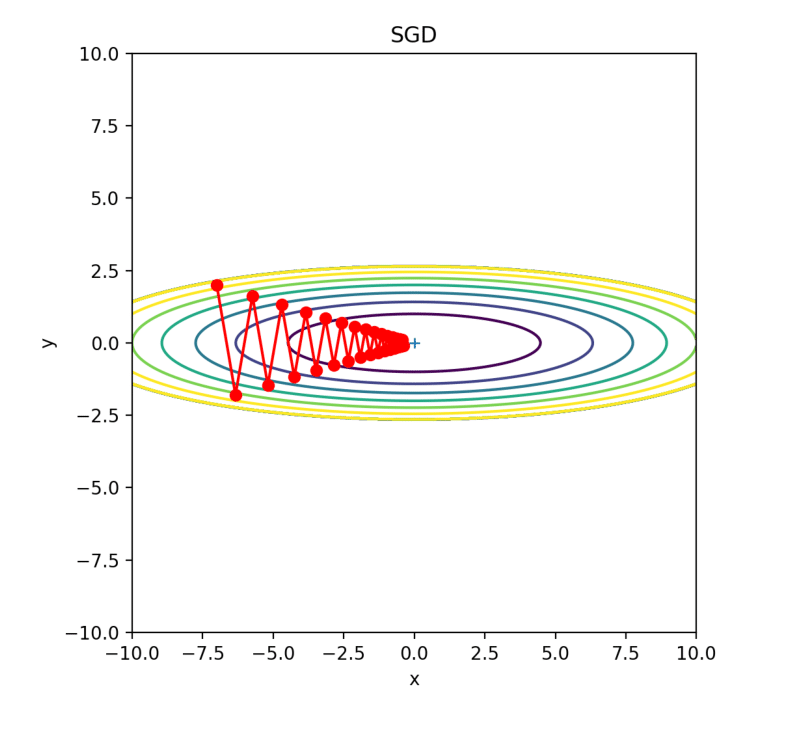
\includegraphics[width=6cm]{./figure/SGD.png}
\caption{SGDによる最適化の更新経路 \label{gr2}}
\end{figure}つまり、確率的勾配下降法の欠点は、関数の形状が等方的出ないと、非効率な経路で探索することになる点にあることがわかる。確率的勾配下降法の非効率な最小値探索経路の原因は、勾配の方向が本来の最小値ではない子方向を指していることにある。そこで、確率的勾配下降法のように単に勾配方向へ進むよりも、より優れた探索方法が求められる。この確率的勾配下降法の欠点を改善するために、Momentum、AdaGrad、Adamという3つの最適化手法を学んだ。
\begin{flushright}
  (※文責:薩田凱斗)
\end{flushright}

}




\subsection{Momentum}
{Momentumは「運動量」という意味の言葉であり、以下のような数式で表される。
\begin{equation}
\label{eq3}
\bf v \leftarrow \alpha v - \eta  \frac{\partial L}{\partial W}
\end{equation}

\begin{equation}
\label{eq4}
\bf W \leftarrow W + v
\end{equation}確率的勾配下降法と同じく、{\bf W}は更新する重みパラメータ、$\displaystyle \frac{\partial L}{\partial W}$は{\bf W}に関する損失関数の勾配、$\displaystyle {\eta}$は学習係数を表す。そして、{\bf v}という変数は速度を表す。式(\ref{eq3})では、物体が勾配方向に力を受け、その力によって物体の速度が加算されるという物理法則を表している。Momentumはボールが地面を転がるような動きに似ている。また、式(\ref{eq3})では、$\displaystyle {\alpha} \bf v$という項があるが、それは物体が何も力を受けないときに徐々に減速するための役割を担っている。物理では、地面の摩擦や空気抵抗に対応する。図\ref{gr3}はMomentumを用いて式(\ref{eq2})の最適化問題を解いた結果である。確率的勾配下降法との大きな違いは、滑らかに最小値に向かっていることである。これは、$\displaystyle x$軸方向に受ける力はとても小さいが、常に同じ方向の力を受けるため、同じ方向へ一定して加速することになる。反対に、$\displaystyle y$軸方向には受ける力は大きいが、正と負の方向の力を交互に受けるため、それらが互いに打ち消し合い、$\displaystyle y$軸方向の速度は安定しない。それゆえ、確率的勾配下降法と比べ、$\displaystyle x$軸方向へと早く近ずくことができ、より滑らかに向かうことができる。
\begin{figure}[H]
\centering
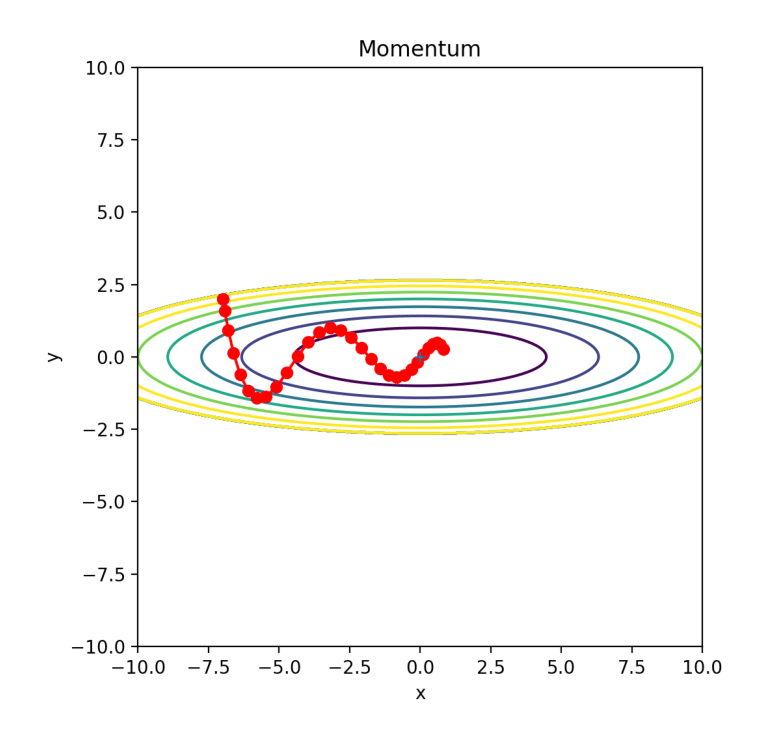
\includegraphics[width=6cm]{./figure/Momentum.png}
\caption{Momentumによる最適化の更新経路 \label{gr3}}
\end{figure}
\begin{flushright}
  (※文責:薩田凱斗)
\end{flushright}
}






\subsection{AdaGrad}
{ニューラルネットワーク の学習では学習係数$\displaystyle {\eta}$の値が重要になる。学習係数が小さすぎると学習に時間がかかりすぎてしまい、逆に大きすぎると発散して正しい学習が行えない。そこで、学習係数に関する有効な方法の1つに学習係数の減衰というものがある。最初に大きく学習し、徐々に小さく学習するというものである。学習係数を徐々に下げていくという考えは、パラメータ全体の学習係数の値を一括して下げることに担当します。これらをさらに発展させたものがAdaGradである。1つ1つのパラメータに対して独自の値を設定する。AdaGradはパラメータの要素ごとに適応的に学習係数を調整しながら学習を行う手法であり、以下のような数式で表される。
\begin{equation} 
\label{eq5}
\bf h \leftarrow  h + \frac{\partial L}{\partial W} \bigodot \frac{\partial L}{\partial W}
\end{equation}

\begin{equation}
\label{eq6}
\bf W \leftarrow W - \eta \frac{1}{\sqrt h}  \frac{\partial L}{\partial W}
\end{equation}確率的勾配下降法と同様に、{\bf W}は更新する重みパラメータ、$\displaystyle \frac{\partial L}{\partial W}$は{\bf W}に関する損失関数の勾配、$\displaystyle {\eta}$は学習係数を表す。ここでは、{\bf h}という変数は式(\ref{eq5})で示されるように、これまでに経験した勾配の値を2乗和として保持する。また、式(\ref{eq5})の$\displaystyle {\bigodot}$は行列の要素ごとの掛け算を意味する。そして、パラメータ更新の際に$\displaystyle \frac{1}{\sqrt h}$を蒸散することで、学習のスケールを調整する。これは、パラメータの要素のなかで大きく更新された要素は、学習係数が小さくなることを意味する。つまり、よく働いたパラメータの学習係数は次第に小さくなるという学習係数の減衰を、パラメータの要素ごとに行うことができる。図\ref{gr4}は、AgaGradを用いて式(\ref{eq2})の最適化問題を解いた結果のグラフである。
\begin{figure}[H]
\centering
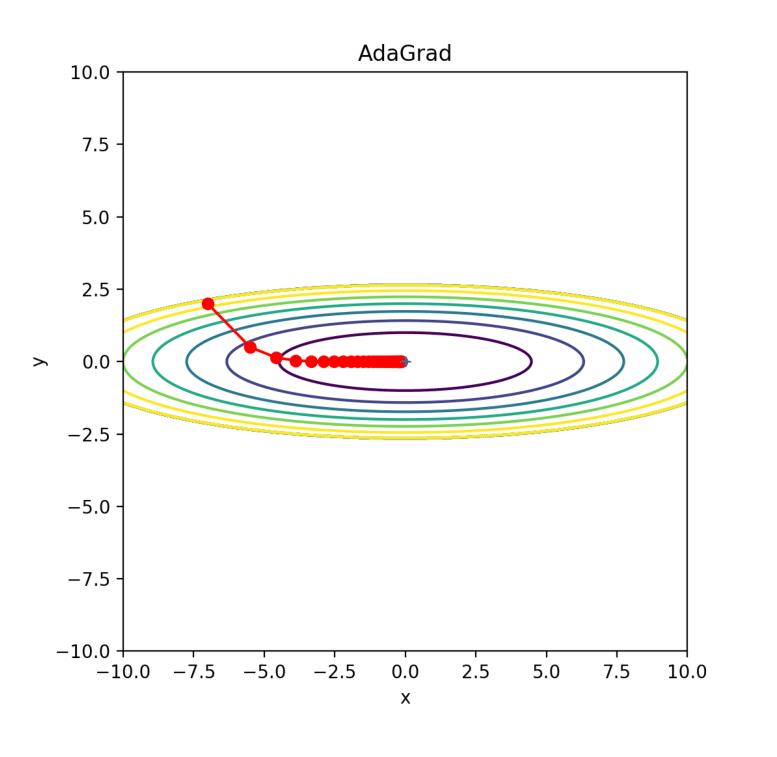
\includegraphics[width=6cm]{./figure/AdaGrad.png}
\caption{AdaGradによる最適化の更新経路 \label{gr4}}
\end{figure}
この結果を見ると、最小値に向かって効率的に動いているのがわかる。$\displaystyle y$軸方向へは勾配が大きいため、最初は大きく動く。その動きに比例し、更新のステップが小さくなるように調整が行われる。そのため、$\displaystyle y$軸方向への更新度合いは弱められていき、滑らかな動きになる。
\begin{flushright}
  (※文責:薩田凱斗)
\end{flushright}
}






\subsection{Adam}
{Adamとは、MomentumとAdaGradを融合した手法であり2015年に提案された新しい手法である。その理論はやや複雑であるが、直感的にはMomentumとAdaGradを融合させ、両者の利点を組み合わせたような探索手法である。この2つの手法を組み合わせることにより、効率的にパラメータ空間を探索することが期待できる。また、ハイパーパラメータのバイアス補正が行われていることもAdamの特徴である。図\ref{gr5}はAdamを用いて式(\ref{eq2})の最適化問題を解いた結果のグラフである。
\begin{figure}[H]
\centering
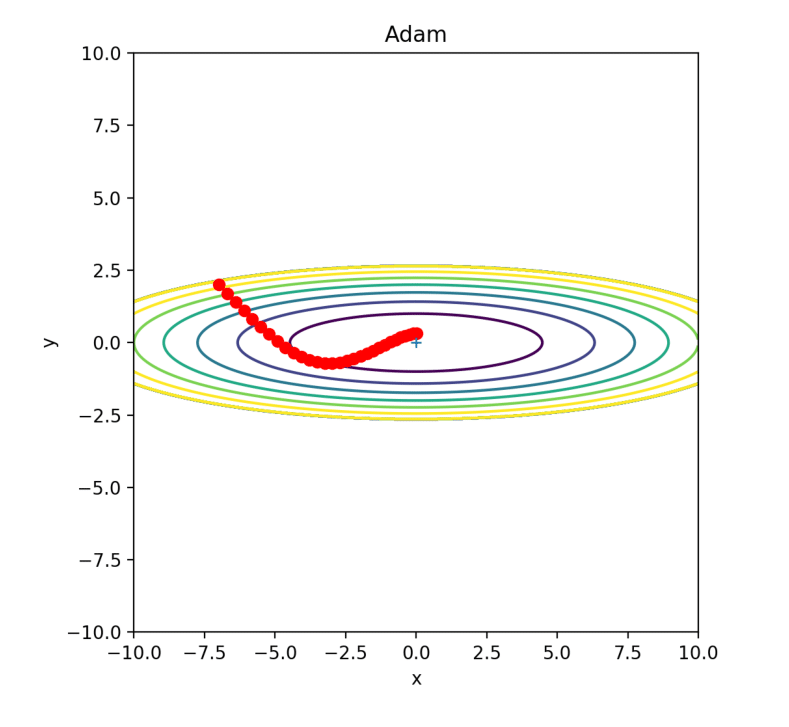
\includegraphics[width=6cm]{./figure/Adam.png}
\caption{Adamによる最適化の更新経路 \label{gr5}}
\end{figure}
図\ref{gr5}で示すように、Adamによる更新の過程は、ボールが転がるような動きをしている。Momentumとも似たような動きをしているが、Momentumよりも左右の揺れが軽減されているのがわかる。これは、学習の更新度合いが適応的に調整されることによってもたらされる。
\begin{flushright}
  (※文責:薩田凱斗)
\end{flushright}
}



\subsection{比較}
{SGD、Momentum、AdaGrad、Adamの4種類のパラメータ更新手法を見てきたわけだが、それぞれに特徴があり、解く問題によって結果が変わってくるので得意な問題、不得意な問題がある。また、ハイパーパラメータ(学習係数)つまり、この手法が最も良い更新手法であるとは一概には言えない。多くの研究ではSGDが今でも使われている。どの手法がより適応しているかを試すためにMomentumやAdaGrad、Adamなども使用してみる価値がある。
\begin{flushright}
  (※文責:薩田凱斗)
\end{flushright}
}
